\section{Deux surfaces}
\begin{enumerate}
  \item \begin{enumerate}
          \item Soit $\alpha\in{R}$
                \[
                  \left\{
                  \begin{array}{r c l}
                    z & = & (y - 2\sqrt{2}x)y \\
                    y & = & \alpha            \\
                  \end{array}
                  \right.
                \]
                \[
                  \Rightarrow
                  \begin{array}{r c l}
                    z & = & (\alpha - 2\sqrt{2}x)\alpha \\
                  \end{array}
                \]
                On reconnaît l'équation d'une droite. Notons-la $D_\alpha$. Alors $S = \bigcup\limits_{\alpha\in\mathbb{R}}^{} D_\alpha$. Par propriété, $S$ est une surface réglée. Ainsi :
                \begin{result}
                  L'intersection de $S$ avec un plan d'éqation $y=\alpha$ est une droite.
                  Alors $S$ est une surface réglée.
                \end{result}
          \item
                Soit $\beta\in\mathbb{R}$, soit $P : x = \beta$, $C = S \bigcap P$.
                On a alors :
                \[
                  \left\{
                  \begin{array}{r c l}
                    z & = & (y - 2\sqrt{2}x)y \\
                    x & = & \beta             \\
                  \end{array}
                  \right.
                \]
                \[
                  \Rightarrow
                  \begin{array}{r c l}
                    z & = & (y - 2\sqrt{2}\beta)y \\
                  \end{array}
                \]
                \[
                  \Rightarrow
                  \begin{array}{r c l}
                    z & = & y^{2} - 2\sqrt{2}\beta y \\
                  \end{array}
                \]
                On reconnaît l'équation d'une parabole.
                Cherchon le point où la courbure est maximale. i.e. $\gamma(t)$ maximale. Passons en équation paramétrique :
                \[
                  \left\{
                  \begin{array}{r c l}
                    y & = & t                        \\
                    z & = & t^{2} - 2\sqrt{2}\beta t \\
                  \end{array}
                  \right.
                \]
                Pour $t\in\mathbb{R}$, posons :
                \[
                  f(t) =
                  \left(
                  \begin{array}{c}
                      t                        \\
                      t^{2} - 2\sqrt{2}\beta t \\
                    \end{array}
                  \right)
                  \Rightarrow
                  f'(t) =
                  \left(
                  \begin{array}{c}
                      1                     \\
                      2(t - 2\sqrt{2}\beta) \\
                    \end{array}
                  \right)
                \]
                Définissons l'angle de relèvement $\alpha$ : \[\forall t\in\mathbb{R}, \alpha(t) = \arctan{(\frac{z'(t)}{y'(t)})}\]
                \[\iff\forall t\in\mathbb{R}, \alpha(t) = \arctan{(2(t-\sqrt{2}\beta))}\]
                Alors :
                \[
                  \forall t\in\mathbb{R},\gamma(t) = \frac{\alpha'(t)}{\left\|f'(t)\right\|}
                \]
                De plus, $\alpha$ est dérivable sur $\mathbb{R}$ :
                \[\forall t\in\mathbb{R}, \alpha'(t) = \frac{2}{1+4(t-\sqrt{2}\beta)^{2}}\]
                Donc :
                \[\forall t\in\mathbb{R}, \gamma(t) = \frac{2}{1+4(t-\sqrt{2}\beta)^{2}}\times \frac{1}{\sqrt{1+4(t-\sqrt{2}\beta)^{2}}}\]
                Ainsi, $\gamma$ est maximal pour $(1+4(t-\sqrt{2}\beta)^{2})^{3/2}$ minimal i.e. $t=\sqrt{2}\beta$

                Ainsi, la courbure $\gamma$ est maximale au point $A(\sqrt{2}\beta, -2\beta^{2})$
                En conclusion :
                \begin{result}
                  La nature de $C$ est une \textbf{parabole}.
                  Le point de $C$ où la courbure est maximale est $\boldsymbol{A(\sqrt{2}\beta, -2\beta^{2})}$
                \end{result}
          \item \begin{enumerate}
                  \item Soit $\gamma \in\mathbb{R}$. On a :
                        \[
                          \left\{
                          \begin{array}{r c l}
                            z & = & (y - 2\sqrt{2}x)y \\
                            z & = & \gamma            \\
                          \end{array}
                          \right.
                          \iff
                          \gamma = (y - 2\sqrt{2}x)y
                        \]
                        On reconnaît alors l'équation d'une conique. On va réduire la conique pour reconnaître
                        une forme canonique et en déduire la nature de $\Lambda_\gamma$.
                        Il est probable\footnote{le \textit{probable} est ici hypocrite : j'ai regardé sur Geogebra... \frownie{}}
                        que la disjonction de cas se fasse dans la partie 3 de la réduction, donnant alors différentes natures
                        de $\Lambda_\gamma$
                        \begin{dinglist}{111}
                          \item
                          \ul{\'{E}tape 1 : r\'{e}duction de la conique}
                          \\ \\
                          Partie quadratique de la conique : $0 \times x^{2} + 2 \times (-\sqrt{2}) xy + 1 \times y^{2}$\\
                          On pose la matrice associée
                          $
                            A =
                            \left(
                            \begin{array}{c c}
                                0         & -\sqrt{2} \\
                                -\sqrt{2} & 1         \\
                              \end{array}
                            \right)
                          $
                          telle que :
                          \[
                            -2\sqrt{2}xy + y^{2} =
                            \left(
                            \begin{array}{c}
                              x \\ y \\
                            \end{array}
                            \right)^{T}
                            A
                            \left(
                            \begin{array}{c}
                              x \\ y \\
                            \end{array}
                            \right)^{T}
                          \]
                          A est symétrique donc diagonalisable dans une base othonormée d'après le théorème spectral.\\
                          Son polynôme caractéristique est :
                          \[
                            x(x-1)=2
                            \iff
                            \left\{
                            \begin{array}{r c l}
                              x & = & -1 \\
                              x & = & 2  \\
                            \end{array}
                            \right.
                          \]\\
                          D'où $Sp=\{-1;2\}$. On pose ainsi $D =
                            \left(
                            \begin{array}{c c}
                                -1 & 0 \\ 0 &  2\\
                              \end{array}
                            \right)
                          $\\
                          On détermine la matrice de passage othogonale $P = \underset{C, B} {mat(Id)}$.\\
                          On détermine les espaces propres pour chaque valeur propre.
                          \begin{dinglist}{111}
                            \item $\lambda = -1$ : \\
                            $E_{(-1)} = ker(A+Id) = ker
                              \left(
                              \begin{array}{c c}
                                  1         & -\sqrt{2} \\
                                  -\sqrt{2} & 2         \\
                                \end{array}
                              \right)
                            $\\
                            Or
                            \[
                              \left(
                              \begin{array}{c c}
                                  1         & -\sqrt{2} \\
                                  -\sqrt{2} & 2         \\
                                \end{array}
                              \right)
                              \underset
                              {L_2 \gets L_2 + \sqrt{2}L_1}
                              {
                                \underset
                                {\mathcal{L}}
                                {\sim}
                              }
                              \left(
                              \begin{array}{c c}
                                  1 & -\sqrt{2} \\
                                  0 & 0         \\
                                \end{array}
                              \right)
                            \]
                            \textit{Remarque : On sait que la matrice est inversible donc on sait que les lignes $L_1$ et $L_2$ sont liées, on n'est donc pas obligé de faire cette étape, mais ça m'a permis de faire des équivalents par ligne sur \LaTeX !}\\
                            Donc
                            \[
                              E_{(-1)} = Vect
                              \left\{
                              \left(
                              \begin{array}{c}
                                  \sqrt{2} \\
                                  1
                                \end{array}
                              \right)
                              \right\}
                            \]
                            Or on veut un vecteur normé. Donc :
                            \[
                              E_{(-1)} = Vect
                              \left\{
                              \frac{1}{\sqrt{3}}
                              \left(
                              \begin{array}{c}
                                  \sqrt{2} \\
                                  1
                                \end{array}
                              \right) = \vec{\varepsilon_1}
                              \right\}
                            \]
                            \item $\lambda = 2$ : \\
                            De manière équivalente on trouve :
                            \[
                              E_{2} = Vect
                              \left\{
                              \frac{1}{\sqrt{3}}
                              \left(
                              \begin{array}{c}
                                  1 \\
                                  -\sqrt{2}
                                \end{array}
                              \right) = \vec{\varepsilon_2}
                              \right\}
                            \]
                          \end{dinglist}
                          \textit{On vérifie rapidement $\vec{\varepsilon_1}.\vec{\varepsilon_2} = 0$}.\\
                          On a alors $P = \frac{1}{\sqrt{3}}
                            \left(
                            \begin{array}{c c}
                                \sqrt{2} & 1         \\
                                1        & -\sqrt{2} \\
                              \end{array}
                            \right)
                          $ et $P^{-1} = P^T = P$. On trouve finalement :
                          \[
                            -2\sqrt{2}xy + y^{2} =
                            \left(
                            \begin{array}{c}
                              x \\ y \\
                            \end{array}
                            \right)^{T}
                            PDP
                            \left(
                            \begin{array}{c}
                              x \\ y \\
                            \end{array}
                            \right)^{T}
                          \]

                          \item
                          \ul{\'{E}tape 2 : Changement de base}\\
                          Soit $M(x, y) \in \Lambda_\gamma$.\\
                          On a alors :
                          $
                            \left(
                            \begin{array}{c}
                                x \\ y \\
                              \end{array}
                            \right)
                            = P
                            \left(
                            \begin{array}{c}
                                X \\ Y \\
                              \end{array}
                            \right)
                          $ avec donc $(X, Y)$ les coordonnées de $M$ dans la base $\mathcal{C} = (\vec{\varepsilon_1}, \vec{\varepsilon_2})$.\\
                          Ainsi, l'équation de la partie quadratique de la conique $\Lambda_\gamma$ devient :
                          \[
                            -2\sqrt{2}xy + y^{2} =
                            \left(
                            \begin{array}{c}
                              x \\ y \\
                            \end{array}
                            \right)^{T}
                            PDP
                            \left(
                            \begin{array}{c}
                              x \\ y \\
                            \end{array}
                            \right)^{T} =
                            \left(
                            \begin{array}{c}
                              X \\ T \\
                            \end{array}
                            \right)^{T}
                            P^{T}PDP^{T}P
                            \left(
                            \begin{array}{c}
                              X \\ Y \\
                            \end{array}
                            \right)^{T} = -X^{2} + 2Y^{2}
                          \]
                          \item
                          \ul{\'{E}tape 3 : Forme canonique}\\
                          \[
                            \Lambda_\gamma : -2\sqrt{2}xy + y^{2} = \gamma
                          \]
                          Comme on a $\alpha\beta\neq0$ :\\
                          \[
                            \left(
                            \begin{array}{c}
                                x \\ y \\
                              \end{array}
                            \right)
                            = \frac{1}{\sqrt{3}}
                            \left(
                            \begin{array}{c c}
                                \sqrt{2} & 1         \\
                                1        & -\sqrt{2} \\
                              \end{array}
                            \right)
                            \left(
                            \begin{array}{c}
                                X \\ Y \\
                              \end{array}
                            \right)
                            \iff
                            \left\{
                            \begin{array}{rcl}
                              x & = & \frac{1}{\sqrt{3}} (\sqrt{2}X+Y) \\
                              y & = & \frac{1}{\sqrt{3}} (X-\sqrt{2}Y) \\
                            \end{array}
                            \right.
                          \]
                          D'où :
                          \[
                            \Lambda_\gamma : 2Y^{2} - X^{2} = \gamma
                          \]
                          Nous avons ainsi notre forme canonique de $\Lambda_\gamma$, et c'est ici qu'apparaît la disjonction de cas sur $\gamma$ :
                          \begin{dinglist}{111}
                            \item $\gamma=0$
                            \[
                              2Y^{2} = X^{2} \iff
                              \left\{
                              \begin{array}{rcl}
                                X & = & \sqrt{2}Y \\
                                X & = & 0         \\
                              \end{array}
                              \right.
                            \]
                            On reconnaît alors deux droites.
                            \item $\gamma\neq0$
                            \[
                              2Y^{2} - X^{2} = \gamma\iff
                              \frac{2}{\gamma}Y^{2} - \frac{X^{2}}{\gamma} = 1
                            \]
                            On reconnaît alors une hyperbole.
                          \end{dinglist}
                        \end{dinglist}
                        Ainsi :
                        \begin{result}
                          $
                            \left\{
                            \begin{array}{rcl}
                              \gamma=0    & \rightarrow & \Lambda_\gamma \text{ est la réunion de 2 droites} \\
                              \gamma\neq0 & \rightarrow & \Lambda_\gamma \text{ est une hyperbole}
                            \end{array}
                            \right.
                          $
                        \end{result}
                  \item
                        Voici le graphe :
                        \begin{center}
                          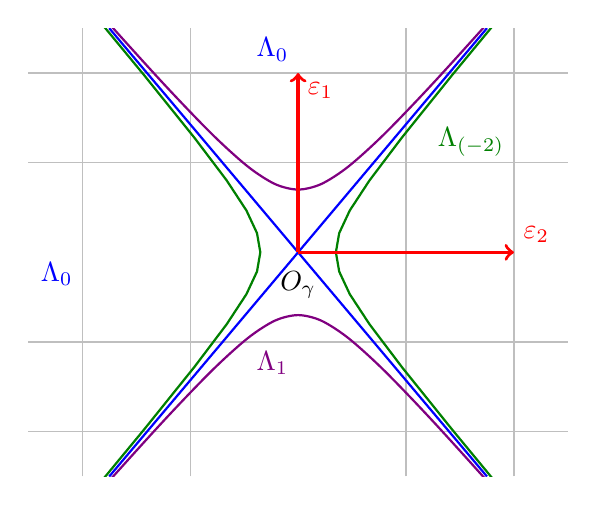
\begin{tikzpicture}
                            \begin{axis} [
                                axis lines=center,
                                axis line style={draw=none},
                                ticks=none,
                                grid=major,
                                xmin=-5,
                                xmax=5,
                                ymin=-5,
                                ymax=5,]
                              \addplot [color=Blue, domain=-5:5, thick] coordinates {(-3.5,-5)(3.5,5)};
                              \addplot [color=Blue, domain=-5:5, thick] coordinates {(3.5,-5)(-3.5,5)};
                              \addplot [Purple,thick,domain=-5:5, smooth] ({sinh(x)}, {1.4*cosh(x)});
                              \addplot [Purple,thick,domain=-5:5, smooth] ({sinh(x)}, {-1.4*cosh(x)});
                              \addplot [Green,thick,domain=-5:5] ({0.7*cosh(x)}, {sinh(x)});
                              \addplot [Green,thick,domain=-5:5] ({-0.7*cosh(x)}, {sinh(x)});
                              \draw[Red,very thick,->](axis cs: 0,0) -- (axis cs: 0,4);
                              \draw (axis cs: 0,4) node [below right, Red] {$\varepsilon_1$};
                              \draw[Red,very thick,->](axis cs: 0,0) -- (axis cs: 4,0);
                              \draw (axis cs: 4,0) node [above right, Red] {$\varepsilon_2$};
                              \draw (axis cs: -4,0) node [below left, Blue] {$\Lambda_0$};
                              \draw (axis cs: 0,5) node [below left, Blue] {$\Lambda_0$};
                              \draw (axis cs: 4,3) node [below left, Green] {$\Lambda_{(-2)}$};
                              \draw (axis cs: 0,-2) node [below left, Purple] {$\Lambda_1$};
                              \draw (axis cs: 0,-0.2) node [below] {$O_\gamma$};
                            \end{axis}
                          \end{tikzpicture}
                        \end{center}
                        \textit{Et bien c'était long à tracer tout ça !}\\
                        \textit{P.S. Je l'avais tracé au brouillon avant, sans aide numérique !}\\
                        \textit{P.S.S. J'ai tout tracé dans la base $C$ pour que ça soit plus simple...}
                \end{enumerate}
          \item
                Soit $\Omega_0(x_0, y_0, z_0)$, $\mathcal{P}$ le plan tangent à S en $\Omega_0$.\\
                Soit $H(x,y,z) \in \mathcal{P}$. Alors $\overrightarrow{\Omega_0H}.\overrightarrow{\nabla}f(\Omega_0)=0$ avec
                $
                  \overrightarrow{\nabla}f(\Omega_0)=
                  \left(
                  \begin{array}{c}
                      -2\sqrt{2}y_0     \\
                      2y_0-2\sqrt{2}x_0 \\
                      -1                \\
                    \end{array}
                  \right)
                $
                \[
                  \iff
                  \left(
                  \begin{array}{c}
                      x-x_0 \\
                      y-y_0 \\
                      z-z_0 \\
                    \end{array}
                  \right).
                  \left(
                  \begin{array}{c}
                      -2\sqrt{2}y_0     \\
                      2y_0-2\sqrt{2}x_0 \\
                      -1                \\
                    \end{array}
                  \right) = 0
                \]
                \[
                  \iff
                  -2\sqrt{2}y_0(x-x_0) + 2(y-y_0)(y_0-\sqrt{2}x_0) - (z-z_0)  0
                \]
                Or $ z_0 = y_0^{2}-2\sqrt{2}x_0y_0$ car $\Omega_0\in S$\\Donc
                \[
                  \iff
                  2\sqrt{2}y_0x + 2(\sqrt{2}x_0-y_0)y + z = 2\sqrt{2}x_0y_0 - y_0^{2}
                \]
                Donc
                \begin{result}
                  L'équation du plan tangeant à $S$ en $\Omega_0$ est :
                  $\boldsymbol{2\sqrt{2}y_0x + 2(\sqrt{2}x_0-y_0)y + z = 2\sqrt{2}x_0y_0 - y_0^{2}}$
                \end{result}
          \item Si $\Omega_0 = O$ alors l'équation devient :
                $z = 0$
                Calculons la matrice hessienne en $O(0,0,0)$ :
                \[
                  H_f(O) = H_f((x, y, z)) = A =
                  \left(
                  \begin{array}{c c}
                      0         & -\sqrt{2} \\
                      -\sqrt{2} & 1         \\
                    \end{array}
                  \right)
                \]
                On remarque que $\overrightarrow{\nabla}f(O) = 0$ donc $O(0,0,0)$ est un point critique. De plus,
                $H_f(O)$ est inversible et ses valeurs propres sont $(\alpha, \beta) = (-1,2)$. Ainsi $\alpha\times\beta<0$. Par théorème, $O$ est un point Col. De plus par propriété :
                \begin{result}
                  $\mathcal{P}$ traverse $S$ en $O$
                \end{result}
        \end{enumerate}
        \begin{enumerate}
          \item
                Soit $M(x, y, z) \in \Sigma$. Montrons que $M\in S$
                \[
                  M(x, y, z) \in \Sigma \Rightarrow
                  \left\{
                  \begin{array}{rcl}
                    x & = & r \times \cos{(\theta)}                            \\
                    y & = & r \times \sin{(\theta)}                            \\
                    z & = & 3 r^{2} \sin{(\theta)}\times\sin{(\theta-\varphi)} \\
                  \end{array}
                  \right.
                \] Or, on remarque que
                \[
                  \begin{array}{rcl}
                    (y-2\sqrt{2}x)y & = & r\sin{(\theta)}(r\sin{(\theta)}-2\sqrt{2}r\cos{(\theta)})   \\
                                    & = & r^{2}\sin{(\theta)}(\sin{(\theta)}-2\sqrt{2}\cos{(\theta)}) \\
                  \end{array}
                \] Or $\varphi = arctan(2\sqrt{2})\iff\tan{(\varphi)}=2\sqrt{2}$ D'où :
                \[
                  \begin{array}{rcl}
                    (y-2\sqrt{2}x)y & = & r^{2}\sin{(\theta)}(\sin{(\theta)}-\tan{(\varphi)}\cos{(\theta)})                                           \\
                                    & = & r^{2}\sin{(\theta)}(\sin{(\theta)}-\frac{\sin{(\varphi)}}{\cos{(\varphi)}}\cos{(\theta)})                   \\
                                    & = & r^{2}\sin{(\theta)}\frac{1}{\cos{(\varphi)}}(\sin{(\theta)}\cos{(\varphi)} - \sin{(\varphi)}\cos{(\theta)}) \\
                                    & = & 3r^{2}\sin{(\theta)}\sin{(\theta - \varphi)}                                                                \\
                                    & = & z                                                                                                           \\
                  \end{array}
                \]Ainsi $M\in S$. Ceci étant vrai pour tout $M\in\Sigma$ :
                \begin{result}
                  $\Sigma \subset S$
                \end{result}
          \item
                Soit $M(x, y, z) \in S$. Montrons que $M\in \Sigma$\\
                On sait que $S$ est une surface réglée donc :
                \[
                  \left\{
                  \begin{array}{rcl}
                    x(\lambda, t) & = & \alpha(t) + \lambda a(t) \\
                    y(\lambda, t) & = & \beta(t) + \lambda b(t)  \\
                    z(\lambda, t) & = & \gamma(t) + \lambda c(t) \\
                  \end{array}
                  \right.
                \] On injecte cela dans l'équation $z=(y-2\sqrt{2}x)$ et on doit pouvoir retrouver les équations paramétriques de $\Sigma$ avec $\lambda = r, t = \theta$, sauf qu'on a du $r^{2}$ dans $z$\dots
                On prouverait alors que $S = \Sigma$.
        \end{enumerate}
        \begin{enumerate}
          \item
                Soit $M(r_0, \theta_0 \in \Sigma$. M est régulier si le vecteur normal au plan tangent à $\Sigma$ en $M$ est non nul.
                Calculons $\overrightarrow{n}$ en $M$ :
                \[
                  \overrightarrow{n} = \frac{\partial f}{\partial r}(r_0, \theta_0) \wedge \frac{\partial f}{\partial \theta}(r_0, \theta_0)
                \]
                \[
                  \frac{\partial f}{\partial r}(r_0, \theta_0) =
                  \left(
                  \begin{array}{c}
                      \cos{(\theta_0)}                               \\
                      \sin{(\theta_0)}                               \\
                      6\sin{(\theta_0)}\sin{(\theta_0 - \varphi)}r_0 \\
                    \end{array}
                  \right)
                \]
                \[
                  \frac{\partial f}{\partial \theta}(r_0, \theta_0) =
                  \left(
                  \begin{array}{c}
                      -r_0\sin{(\theta_0)}                                                                              \\
                      r_0\cos{(\theta_0)}                                                                               \\
                      3r_0^{2}(\cos{(\theta_0)}\sin{(\theta_0 - \varphi)} + \sin{(\theta_0)}\cos{(\theta_0 - \varphi)}) \\
                    \end{array}
                  \right) =
                  \left(
                  \begin{array}{c}
                      -r_0\sin{(\theta_0)}                \\
                      r_0\cos{(\theta_0)}                 \\
                      3r_0^{2}\sin{(2\theta_0 - \varphi)} \\
                    \end{array}
                  \right)
                \]
                \[
                  \overrightarrow{n} =
                  \left(
                  \begin{array}{c}
                      3r_0^{2}\sin{(2\theta_0 - \varphi)}\sin{(\theta_0)} - 6\sin{(\theta_0)}\sin{(\theta_0 - \varphi)}r_0 \times r_0\cos{(\theta_0)}      \\
                      6\sin{(\theta_0)}\sin{(\theta_0 - \varphi)}r_0 \times  r_0\sin{(\theta_0)} + r_0\cos{(\theta_0)} 3r_0^{2}\sin{(2\theta_0 - \varphi)} \\
                      r_0\cos^{2}{(\theta_0)} + r_0\sin^{2}{(\theta_0)}                                                                                    \\
                    \end{array}
                  \right)
                \]
                \[
                  \overrightarrow{n} = r_0^{2}
                  \left(
                  \begin{array}{c}
                      3\sin{(\theta_0)}\left[ \sin{(2\theta_0 - \varphi)} - 2\sin{(\theta_0 - \varphi)}\cos{(\theta_0)}\right]       \\
                      3\left[ 2\sin^{2}{(\theta_0)}\sin{(\theta_0 - \varphi)} + \cos{(\theta_0)} \sin{(2\theta_0 - \varphi)} \right] \\
                      1                                                                                                              \\
                    \end{array}
                  \right)
                \]
                Alors $\overrightarrow{n} = 0$ pour $r = 0$
                Ainsi le seul point non régulier de $\Sigma$ est $O$.
                \begin{result}
                  L'ensemble des points non réguliers de $\Sigma$ est le point $O(0, 0, 0)$
                \end{result}
          \item
                Soit $M(r, \theta)\in\Sigma$. Soit $H(x, y, z)\in\mathcal{P}$ avec $\mathcal{P}$ le plan tangent à $\Sigma$ en $M$.
                Alors, $\overrightarrow{MH}.\overrightarrow{n} = 0$ :
                \[
                  \iff r^{2}
                  \left(
                  \begin{array}{c}
                      3\sin{(\theta_0)}\left[ \sin{(2\theta_0 - \varphi)} - 2\sin{(\theta_0 - \varphi)}\cos{(\theta_0)}\right]       \\
                      3\left[ 2\sin^{2}{(\theta_0)}\sin{(\theta_0 - \varphi)} + \cos{(\theta_0)} \sin{(2\theta_0 - \varphi)} \right] \\
                      1                                                                                                              \\
                    \end{array}
                  \right) .
                  \left(
                  \begin{array}{c}
                      x-r\cos{(\theta)}                             \\
                      y-r\sin{(\theta)}                             \\
                      z-r^{2}\sin{(\theta)}\sin{(\theta - \varphi)} \\
                    \end{array}
                  \right) = 0
                \]On trouve alors :
                \begin{result}
                  \textit{Développer les calculs...}
                \end{result}
        \end{enumerate}
\end{enumerate}
